As the purpose of the project is to create a system in which a user should be able to see the weather forecast for a specific area, or more precisely, the temperature forecast, we have developed a system that leverages several models to perform the temperature forecasting. 
The goal is to allow the user to interact with the system in such a way that the user can see the accuracy of the different models. 
The user is able to select a city for which they want to predict the temperature. The results are shown both as a graph that displays the predicted value versus the actual value, as well as the specific set of temperatures of that city for a given time period into the future. This is similar to what one may see on regular weather forecasts.

In order to achieve, this we have constructed a pipeline that preprocesses the data, trains our models, and the resulting models are then used to perform the forecasting displayed on a web application. 
Figure \ref{fig:architecture diagram} shows an overview of the architecture of the pipeline.

\begin{figure*}
	\centering
	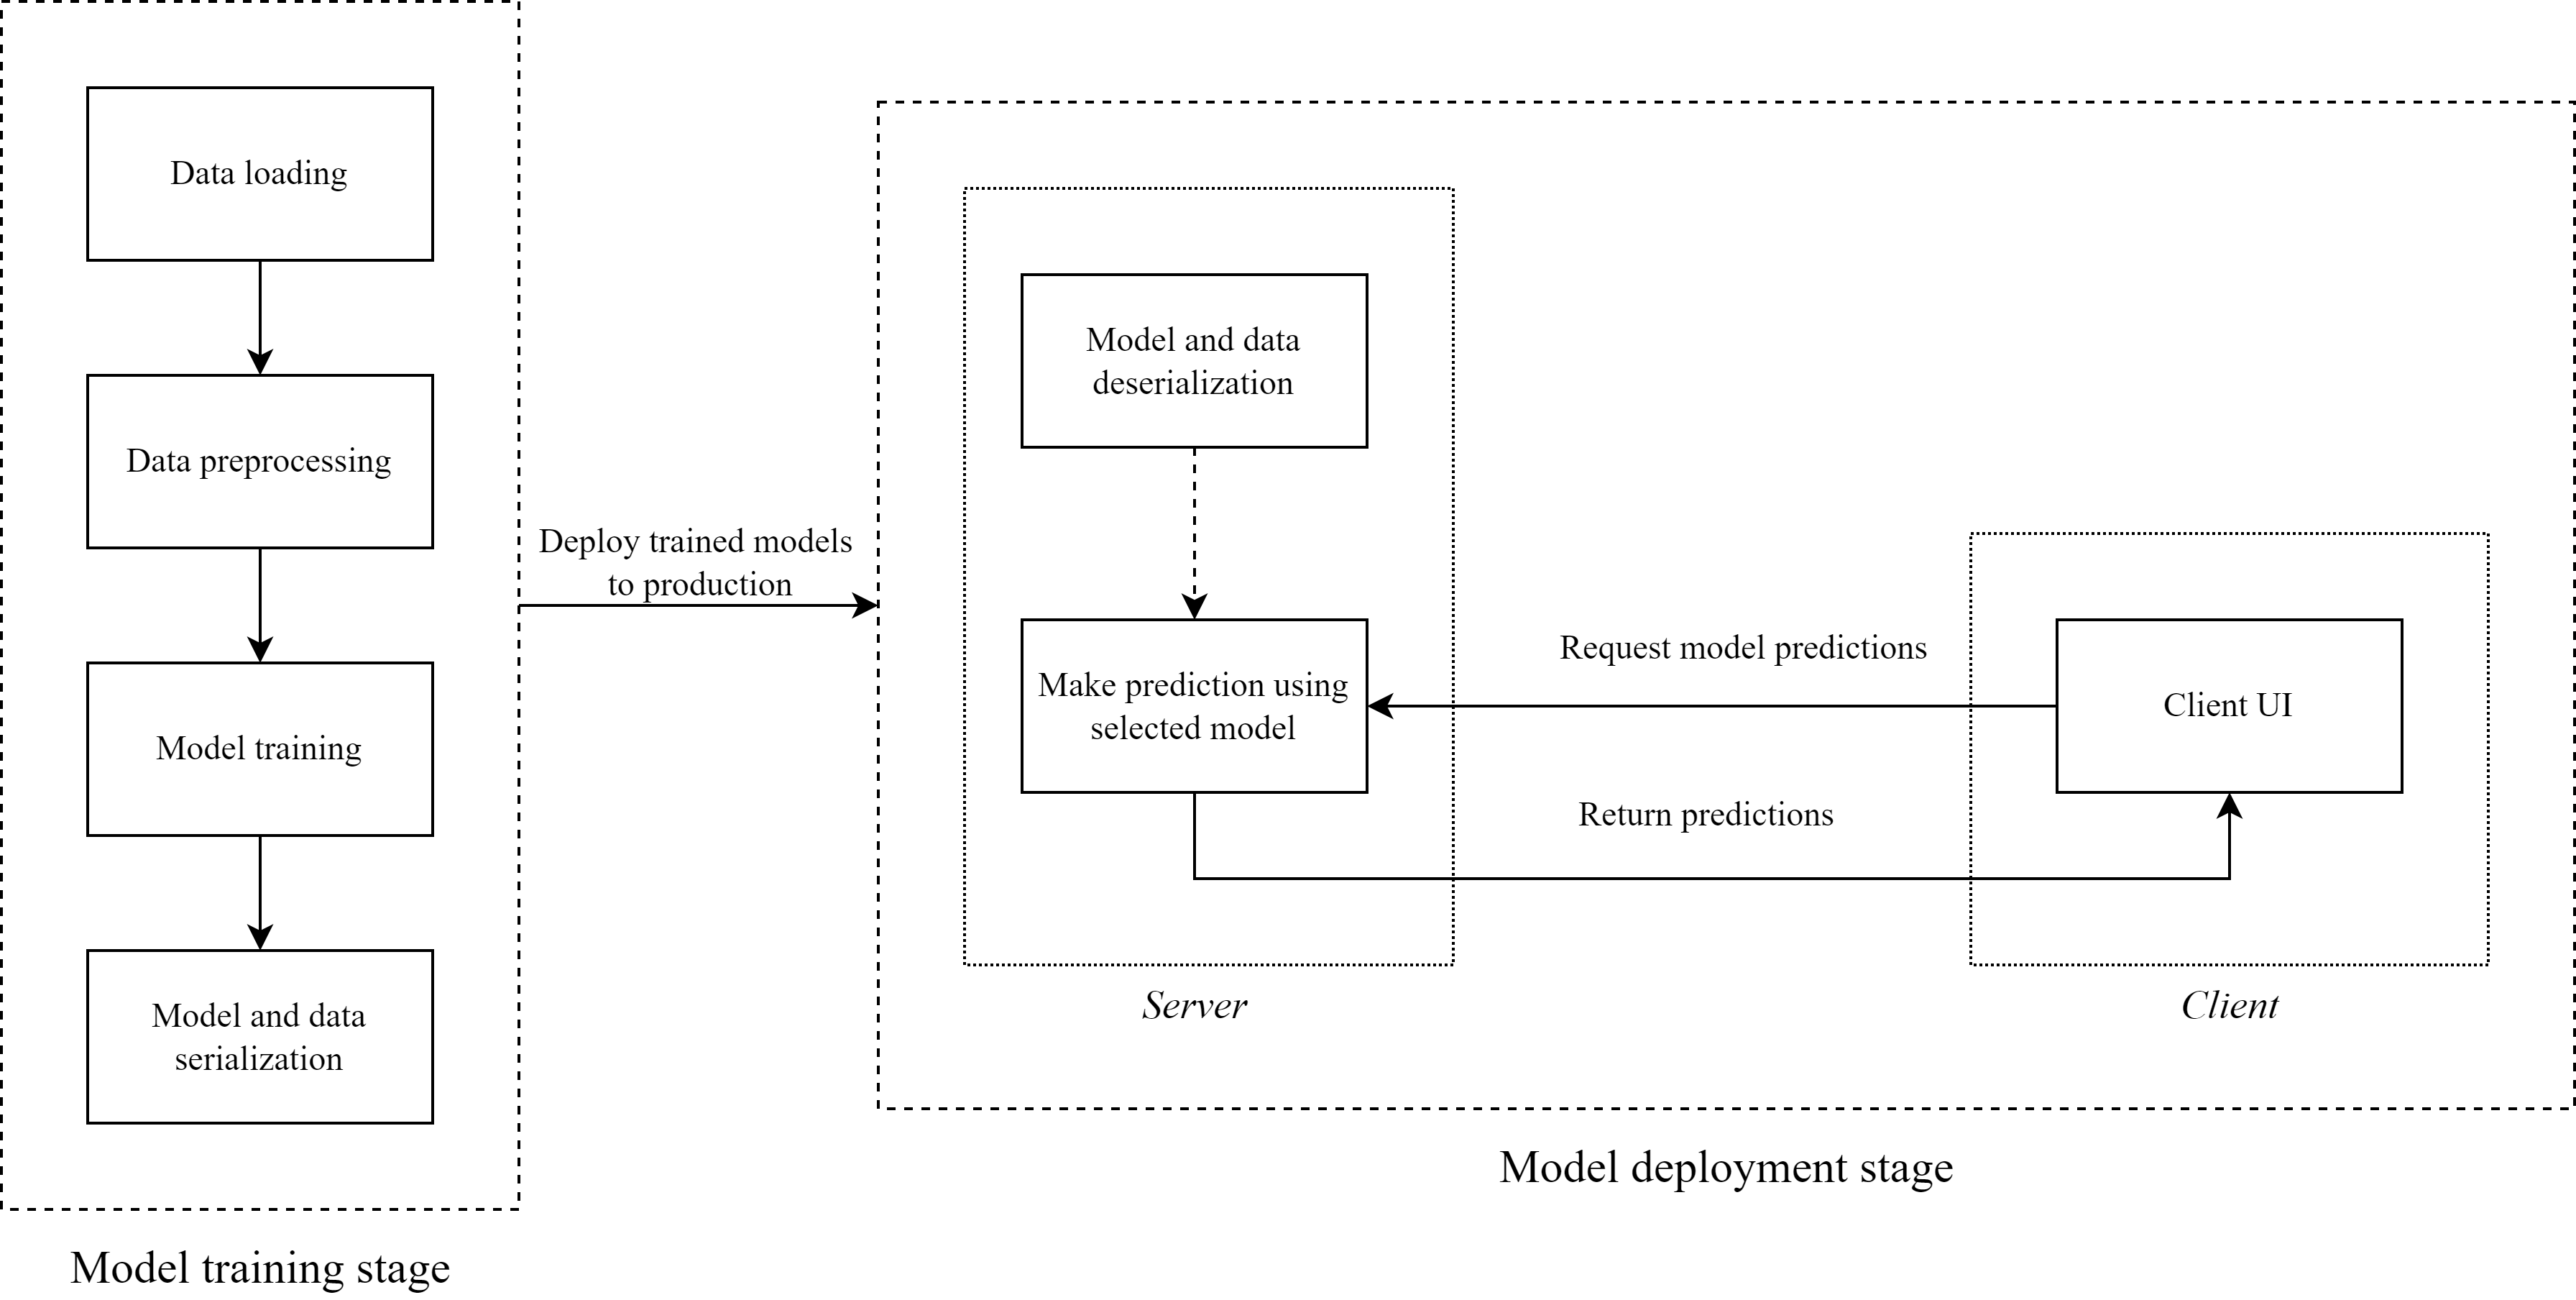
\includegraphics[width=0.85\textwidth]{Architecture diagram}
	\caption{The architecture of the system pipeline.}
	\label{fig:architecture diagram}
\end{figure*}

\subsection{Data loading and preprocessing}
In order to load the data, we use the Pandas library for Python.
Data are loaded from CSV files and then passed to the preprocessing stage.

Preprocessing is done by first stripping the Pandas DataFrame of all columns except the target column $y$. In our case, this is the column denoting the temperature.

Next, we add $n$ time lag features. Let $x_{t,y}$ denote value of the target attribute $y$ at time step $t$ for $N$ sensors. 
Time lag features are added by adding $L=\{1,\dots, n\}$ attributes where $L_{i=1}^n=x_{t-i, y}$ for each $x_{t}$.```

As we used different Python frameworks for different models, the processing from here depended on the framework. Some models required the dataset to be converted to tensors, and others did not.
Besides this, we also split the data into test and training sets with a $0.33/0.77$ distribution for testing and training, respectively.